\section{Serverless Architecture}\label{sec:architecture}

According to~\cite{Roberts}, the deployed serverless architecture make extensive use of third parties services, or "\emph{as-a-Service}-like" components, that replace ad-hoc software and hardware and fulfill the same tasks. In particular we have been able to delegate the following aspects to external and specialized services: application distribution, user management, model generation (heavy computation), user collaboration and state storage.


\subsubsection*{Distribution}
%distribution of the web application => webserver => CDN (keycdn)

To serve the application resources (JavaScript files, images, etc.) we rely on a keycdn CDN\footnote{\url{https://www.keycdn.com/}} (Content Delivery Network) and avoid any kind of webserver. This implies high availability and performance, but also represents a centralized method to upgrade client application without any user explicit action: once files have been updated on the CDN, at the subsequent reload of the web application, any user is provided with the updated version of the application.

\subsubsection*{User Management}
%user management => backend => Backend-as-a-Service (Auth0)

User management activities, which requires a backend running code to accomplish user subscription and authentication, are delegated to Auth0\footnote{\url{https://auth0.com/}}, a Backend-as-a-Service (BaaS) specialized on accounting.

\subsubsection*{Model Generation}
% 3D model generation of heavy building elements => backend => Function-as-a-Service (AWS lambda)

The generation of 3D models may require a while. In that case, especially on low-performing hardware, the computation can't be performed on the client-side, but rather on a powerful server which generate the model on demand, taking as input the parametrization made by the user through the web interface. On this purpose we chose to move this computation on AWS Lambda\footnote{\url{https://aws.amazon.com/lambda/}}, a Function-as-a-Service (FaaS) on which runs the Python code responsible to generate 3D models, that automatically scale on the basis of the number of model generation tasks.

\subsubsection*{Users Collaboration}
% users collaboration => backend => Backend-as-a-Service (Firebase)

As regard the users collaboration, it requires some sort of synchronization among them. To use a single point of synchronization results in a much simpler architecture, so instead of relay on complex peer-to-peer architecture, which however would be a good choice aligned with the serverless paradigm we are pursuing, we opted for a synchronization mechanism based on Firebase\footnote{\url{https://firebase.google.com/}}, a Backend-as-a-Service working as a coordination manager. It broadcasts each change made by a user to all the others. Conflicts are avoided exploiting layers: each user lock the layer she is working on.

\subsubsection*{State Storage}
% state storage =>  DB => Orchestrate.io\footnote{\url{https://orchestrate.io}}

%\iffalse
%The whole state of a modeling project is represented as a JSON document. To save and reload project state we relay on a DataBase-as-a-Service (DBaaS), Orchestrate\footnote{\url{https://orchestrate.io/}} specifically. We only exploited endpoints to save and load a document: on a save event,  client application serializes the centralized state and passes it to the DBaaS which store it, ready to serve it on a load request. Once the client receives the document, the state is automatically restored thanks to its reactive architecture.
%Instead of the DBaaS, the user can even download the serialized JSON state on her hard-drive and upload it again at a later time. The focus here is not on the service that actually store the document, which as stated can be replaced even with a file download, but more precisely, on the software architecture that supports serialization and a reloading of the state. This architecture addresses two main concerns: (i) centralized immutable state and (ii) a reactive characterization (i.e. modification of the state reflects automatically on the user interface).
%\fi

The whole state of a modeling project is represented as a JSON document. To save and reload project state the user can easily downloads the corresponding JSON document, or, to remain ``in the Cloud'', the same document can be stored on a DataBase-as-a-Service (DBaaS), Orchestrate\footnote{\url{https://orchestrate.io/}} for example. In this case we only relay on endpoints to save and to load a document: on a save event,  client application serializes the state and passes it to the DBaaS which store it, ready to serve it on a load request issued at a later time. Once the client receives back the document, the state is automatically restored thanks to its reactive architecture.


The real support for serverless architecture is here not provided by the service that actually store the document, which as stated can be replaced even with a file download, but more precisely, by the software architecture that supports serialization and a reloading of the state. This architecture addresses two main concerns: (i) centralized immutable state and (ii) a reactive UI (i.e. modifications of the state reflect automatically on the user interface).

\subsection{Centralized Application State}\label{ssub:centr_state}

The application state is modeled using the data structure shown in Listing~\ref{lst:structure}. It is essentially a collection of layers, each containing a collection of vertices, lines, areas and objects, each one of which is captured in a structure composed by: (i) information required by the object prototype; (ii) references mapping the relationship to other objects; (iii) metadata, namely the object customization entry point. Listings~\ref{lst:vertex} and \ref{lst:line} give examples of data structures adopted to model a vertex and a line, respectively. 

Information redundancies are exploited to decrease access times. Collections of objects are indexed by \texttt{id} thus allowing lookup in constant time, The \texttt{selected} field of each layer, whose contained information is already present in each object,  grants direct access to selected elements, without searching.

The state can be loaded one layer at a time to support state fragmentation thus allowing to deal with very big building modeling project.

\begin{listing}
\begin{minted}[
               baselinestretch=1,
               fontsize=\footnotesize,
               frame=single,
               framesep=1mm,
               linenos=true,
               xleftmargin=16pt,
               tabsize=2]{js}
{
  "width": 3000, // canvas width
  "height": 2000, // canvas height
  "unit": "cm",  // unit of measurement
  "selectedLayer": "layer-1", // current layer
  "layers": {
    "layer-1": {
      "name": "default",
      "id": "layer-1",
      "altitude": 0,
      "opacity": 1,
      "visible": true,
      "vertices": {
        "HJAe59YF8Ux": {...}
        // ...
      },
      "lines": {
        "Hype99FK88x": {...}
        // ...
      },
      "openings": {
        "r1jaKYUIg": {...}
        // ...
      },
      "areas": {
        "Byg1oFKUIe": {...}
        // ...
      },
      "items": {
        "rkKU89U8e": {...}
        // ...
      },
     //selected element
      "selected": {
        "vertices": [],
        "lines": [],
        "openings": [],
        "areas": [],
        "objects": ["rkKU89U8e"]
      }
    }
  }
}
\end{minted}
\caption{JSON serialized state, overall structure} 
\label{lst:structure}
\end{listing}

\begin{listing}
\begin{minted}[
               baselinestretch=1,
               fontsize=\footnotesize,
               frame=single,
               framesep=1mm,
               linenos=true,
               xleftmargin=16pt,
               tabsize=2]{js}
{
  "id": "HJAe59YF8Ux",
  "x": 201,
  "y": 891,
  "prototype": "vertices",
  "selected": false,
  "lines": ["Hype99FK88x", "S1w-hqKKL8e"],
  "areas": ["Byg1oFKUIe"]
}
\end{minted}
\caption{JSON serialized state, {\tt vertex} structure} 
\label{lst:vertex}
\end{listing}

\begin{listing}
\begin{minted}[
               baselinestretch=1,
               fontsize=\footnotesize,
               frame=single,
               framesep=1mm,
               linenos=true,
               xleftmargin=16pt,
               tabsize=2]{js}
{
  "id": "Hype99FK88x",
  "type": "linear",
  "prototype": "lines",
  "vertices": ["HJAe59YF8Ux", "r11Z59tKIUg"],
  "openings": ["r1jaKYUIg", "BJVZ2M9FIIx"],
  "selected": false,
  "properties": {
    "height": 300,
    "thickness": 20,
    "coverA": "bricks",
    "coverB": "bricks"
 }
\end{minted}
\caption{JSON serialized state, {\tt line} structure} 
\label{lst:line}
\end{listing}

%%%%%%%%%%%%%%%
\iffalse

\begin{listing}
\begin{minted}[
               baselinestretch=1,
               fontsize=\footnotesize,
               frame=single,
               framesep=1mm,
               linenos=true,
               xleftmargin=16pt,
               tabsize=2]{js}
"r1jaKYUIg": {
  "id": "r1jaKYUIg",
  "type": "sash window",
  "prototype": "openings",
  "offset": 0.1873,
  "line": "Hype99FK88x",
  "selected": false,
  "properties": {
    "width":  90,
    "height": 100,
    "altitude": 90,
    "thickness": 10
    }
  }
}
\end{minted}
\caption{JSON serialized state, {\tt opening} structure} 
\label{lst:opening}
\end{listing}



\begin{listing}
\begin{minted}[
               baselinestretch=1,
               fontsize=\footnotesize,
               frame=single,
               framesep=1mm,
               linenos=true,
               xleftmargin=16pt,
               tabsize=2]{js}
"Byg1oFKUIe": {
  "id": "Byg1oFKUIe",
  "type": "area",
  "prototype": "areas",
  "vertices": ["rJO-2qFt8Ue", "HJAe59YF8Ux", "r11Z59tKIUg", "S1VRqtYLIg"],
  "selected": false,
  "properties": {
    "patternColor": "#f5f4f4",
    "texture": "parquet"
  }
}
\end{minted}
\caption{JSON serialized state, {\tt area} structure} 
\label{area}
\end{listing}




\begin{listing}
\begin{minted}[
               baselinestretch=1,
               fontsize=\footnotesize,
               frame=single,
               framesep=1mm,
               linenos=true,
               xleftmargin=16pt,
               tabsize=2]{js}
"rkKU89U8e": {
  "id": "rkKU89U8e",
  "prototype": "items",
  "type": "wardrobe",
  "properties": {
    "width":  200,
    "height": 150
  },
  "selected": false,
  "x": 609,
  "y": 1624,
  "rotation": 1.15
}
\end{minted}
\caption{JSON serialized state, {\tt item} structure} 
\label{lst:item}
\end{listing}

\fi
%%%%%%%%%%%%%%%



\iffalse
%\subsubsection*{Unidirectional data flow} The application exploits the \textbf{unidirectional data flow pattern} to gain great benefits in terms of maintainability of the software objects, due to the lightness of the resulting architecture. As requested by the pattern, the software has to be based on a \textbf{centralized state}, which represents the application logic. Consequently, every feature has as its unique goal the obtainment of a new state coherent with the requested change, following various mechanisms based on \textbf{actions} (each one containing the data for the new state) and \textbf{reducers} (software objects that can write the new state) provided by the \textbf{Redux.js}\footnote{\url{http://redux.js.org/}} library. Usually, the unidirectional data flow pattern is associated with the \textbf{Immutability pattern}, which contributes to maintainability, avoiding side effects for state changes and providing smaller tests for application logic changes. We also benefits of undo/redo operations to an oldest/newer state by means of a replacement of the current state with the previous/next one. As a consequence, the state can be seen as an \textbf{immutable tree structure} whose changes require: (i) The build of a new state \texttt{s'} equal to the previous state \texttt{s}; (ii) Execution of changes on the new state \texttt{s'}; (iii) Reference replacement from \texttt{s} to \texttt{s'}. Despite its simplicity, this pattern can nevertheless lead to memory waste, so we used the \textbf{Immutable.js}\footnote{\url{https://facebook.github.io/immutable-js/}} library (made by facebook), which exploits structural sharing via hash maps tries and vector tries minimizing the need to copy or cache data.
\fi



\subsubsection*{Unidirectional data flow} The described data structure represents the centralized state required by the \emph{unidirectional data flow pattern}~\cite{CITARE QUALCOSA} exploited by the application via \emph{Redux.js}\footnote{\url{http://redux.js.org/}} library. The pattern prescribes that the state may be modified only by specific actors, called \emph{reducers}, whose action is triggered by specific \emph{actions} which contain all the information needed by each reducer to accomplish the state change. Each application feature has to be implemented therefore as a couple of well isolated pieces of code $($ \emph{action} / \emph{reducer} $)$. Preliminary experiments\footnote{\url{https://github.com/cvdlab/walle}} on 2D drawing tools, in fact, highlighted the development complexity of an application of this kind in terms of large internal state modified by several user interactions, which was to be listened to and applied, resulting in a high coupling level between application logic and user interface. In our setup instead we defined a \emph{state engine}, which represents the application logic, comprising actions and reducers, and encapsulates the centralized state. On this layer can transparently relay different interfaces.


\subsubsection*{Immutability pattern} \emph{Immutability pattern}~\cite{CITARE QUALCOSA} is also applied, to avoid side effects on state changes performed by reducers. The state can be seen as an immutable tree structure whose changes are applied as follows: (i) clone the previous state \texttt{s} obtaining a new state \texttt{s'}; (ii) apply changes on the cloned state \texttt{s'}; (iii) Update reference from \texttt{s} to \texttt{s'}. It is worth noting that this approach provides out-of-the-box support for undo/redo operations: an oldest/newer state can be restored by means of a replacement of the current state with the previous/next one.


Despite its simplicity, this pattern can nevertheless lead to memory waste, due to the several copies of the state that must be held in memory. We addressed this issue using \textbf{Immutable.js}\footnote{\url{https://facebook.github.io/immutable-js/}}, a library which exploits structural sharing via hash maps tries and vector tries, thus minimizing the need to copy or cache data.



% FSM
\subsubsection*{User interaction} We modeled the user interaction as a \emph{Finite State Machine} (FSM) where each node corresponds to a \emph{mode} (i.e. to a possible application state), and each edge corresponds to an action (e.g. a user interaction) that can be set off in the current state, (typically a JavaScript event mapping a user interaction such as \texttt{click} or \texttt{mousemove}). 

Figure~\ref{fig_uc_draw_wall} shows the FSM relative to the wall drawing interaction. How we can see there are three nodes corresponding to three modes: (i) Node \texttt{idle}: waiting mode of the application. No action has been taken yet. (ii) Node \texttt{waiting\_drawing\_wall}: user has selected wall design tool, but he hasn't started the draw phase yet. (iii) Node \texttt{drawing\_wall}: user has placed the starting point of the wall.


\begin{figure}[!t]
\centering
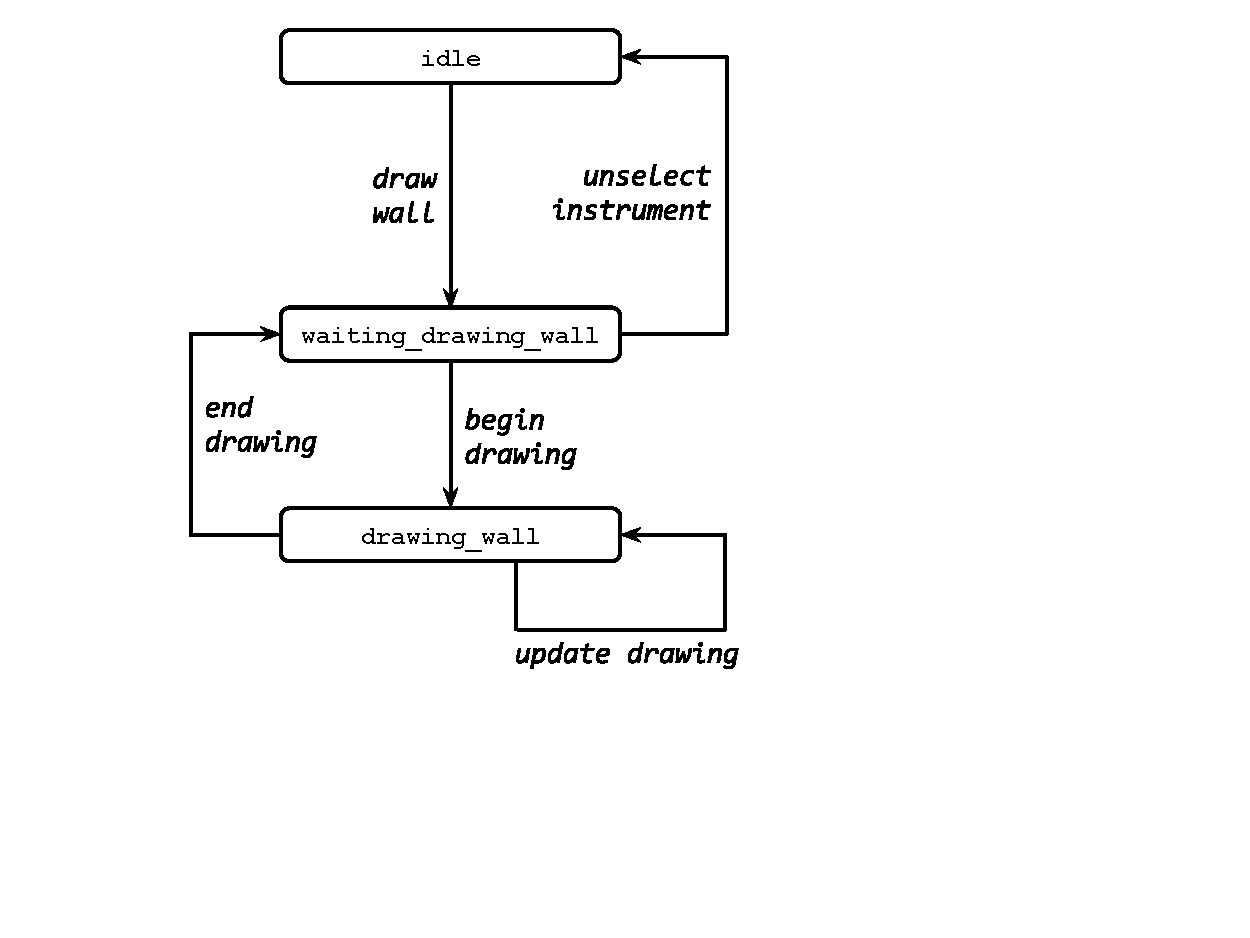
\includegraphics[width=0.6\linewidth]{contents/images/uc_draw_wall}

\caption{Subgraph of the state machine that show a wall creation.}
\label{fig_uc_draw_wall}
\end{figure}



\subsection{Reactive Component Based UI}

The UI has been developed following the \emph{Web Components pattern}~\cite{CITARE-QUALCOSA}, supported by \emph{React.js}\footnote{https://github.com/facebook/react} framework. The main idea is to define the frontend application as a collection of independent components, each one referencing a specific subset of the centralized state and able to render itself according to the actual values of that portion of the state. Web Components spawn from for high level generic containers, like the toolbar or the catalog, to very fine grained ones, buttons for example. The most interesting are the viewers of the building model: the \emph{2D-viewer} and the \emph{3D-viewer}.

\subsubsection*{Viewers} A viewer is a pivotal component since it shows the building model and allows user interaction with it. We built a \emph{2D-viewer} and a \emph{3D-viewer}. 

The \emph{2D-viewer} invokes the \emph{2Dgf} of the building elements added to the model and renders its output using SVG elements. To cope with frequent updates coming from the user drawing interaction, it exploits the \emph{Virtual DOM}~\cite{vdom}, which permits to update only the modified part thus avoiding complete redrawing of the scene. To perform pan and zoom operations, typically necessary in this kind of tool, we develop an ad-hoc React component named \emph{ReactSVGPanZoom}\footnote{https://github.com/chrvadala/react-svg-pan-zoom}.



The latter offers two interaction ways: a 3D model can be inspected from the outside as well as walking inside it in a first-person point-of-view.


The \emph{3D-viewer} invokes the \emph{3Dgf} of the building elements added to the model and renders its output using WebGL primitives via \textbf{Three.js}~\footnote{https://threejs.org/}. Iit has been implemented a \texttt{diff} and \textit{patch} system, standardized in~\cite{rfc6902}: Three.js objects are associated with building elements inside the state, so every time the user triggers an action that results in a state alteration, the application compute the difference between the old state and the new one a thus change only the affected object. In particular we can have the following \textit{operations}: (i) \textbf{add}, (ii) \textbf{replace} and (iii) \textbf{remove}.


Figure~\ref{fig_viewers} shows the interaction among viewers, state-engine and catalog. A viewer reacts to any state change updating its internal state and displaying the changes applied to the model. The generating function are pulled from the catalog where a descriptor for each building elements can be found.


\begin{figure}[htb]
\centering
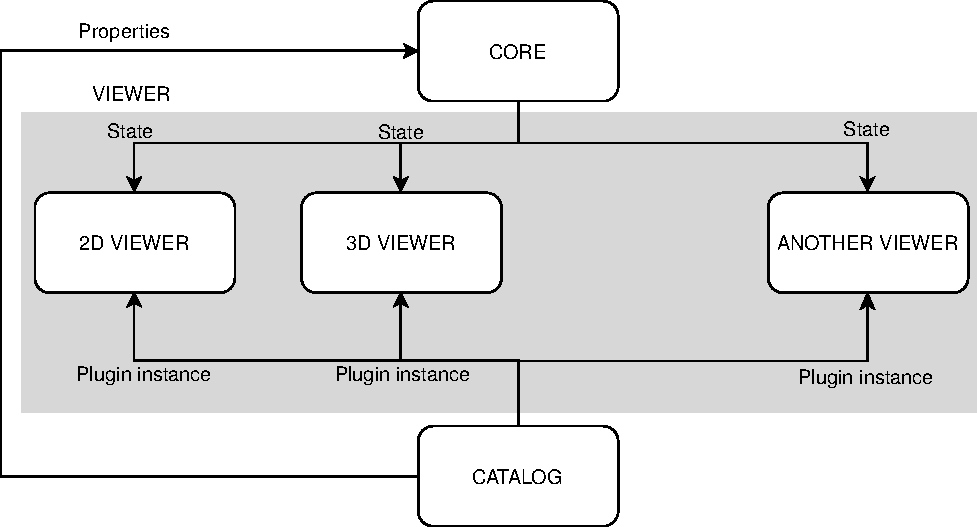
\includegraphics[width=\linewidth]{contents/images/diagramma-visualizzatori}
\caption{Viewers architectural scheme}
\label{fig_viewers}
\end{figure}

\begin{figure}[htb]
\centering
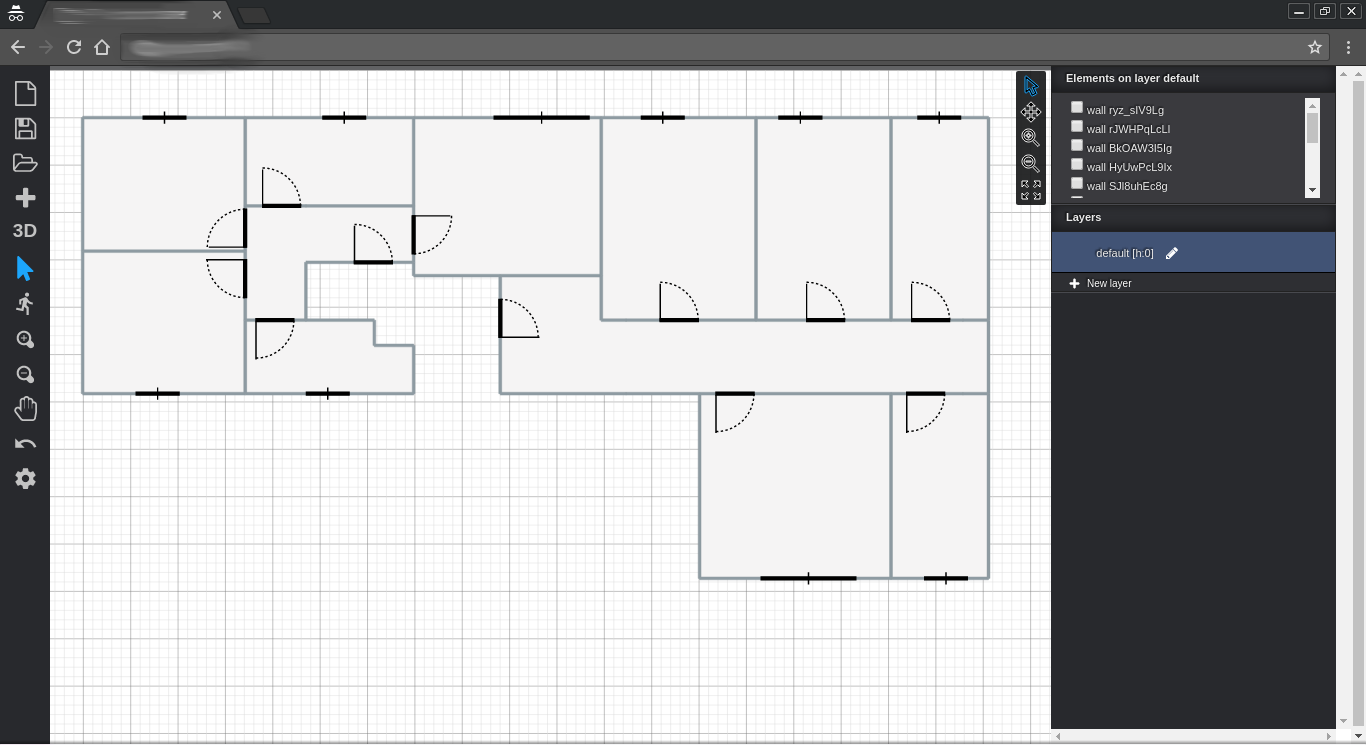
\includegraphics[width=0.45\linewidth]{contents/images/fig-pianta}
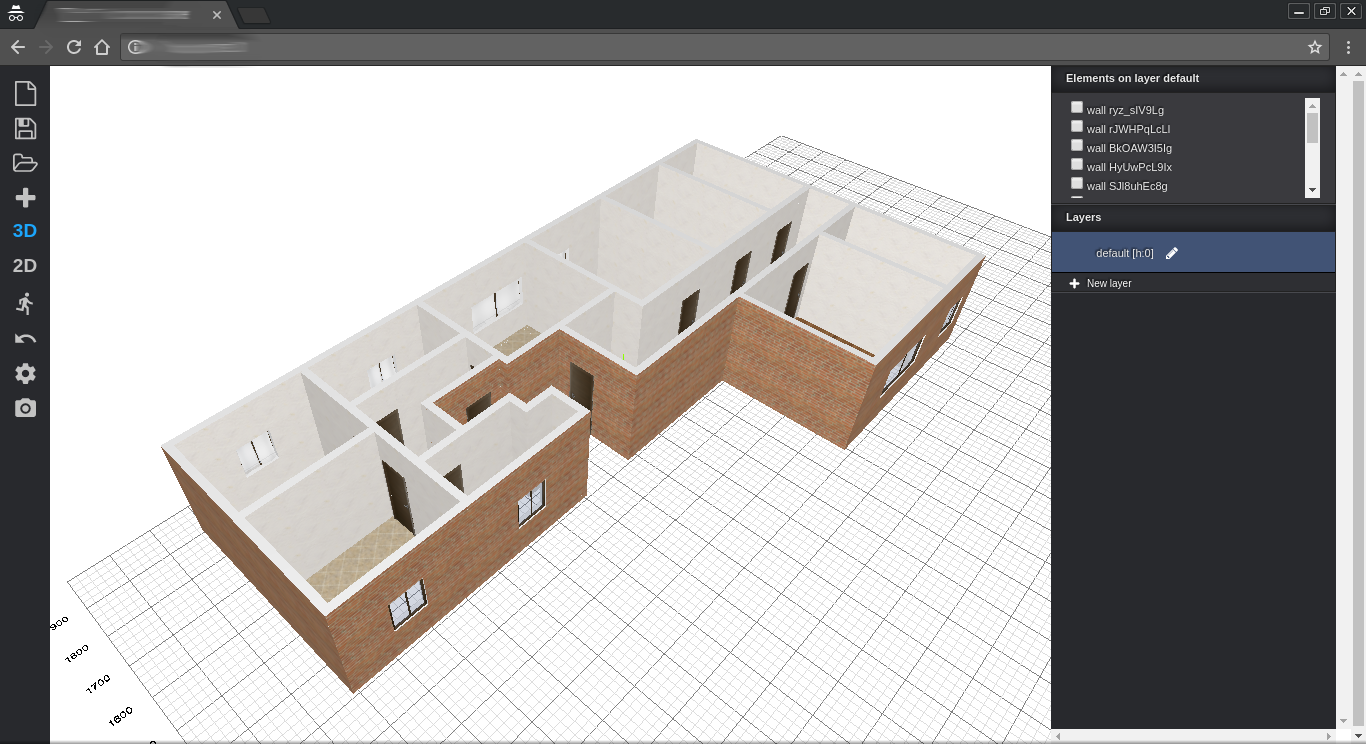
\includegraphics[width=0.45\linewidth]{contents/images/fig-pianta-3d}
\caption{The 2D and 3D viewers for the state}
\label{fig_viewer}
\end{figure}


